\documentclass{article}
\usepackage{graphicx}
\usepackage{listings}
\begin{document}

\section{Using Figure 2.2 as a model? illustrate the operation of Insertion-Sort on the array A = (31,41,59,26,41,58).}
\begin{figure}[!htb] 
  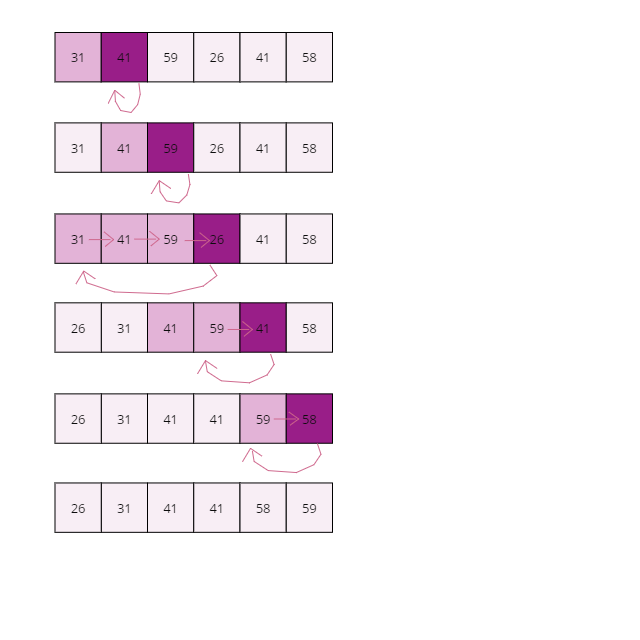
\includegraphics[width=\textwidth]{2_1-1.png}
\end{figure}
 
\section{Rewrite the Insertion-Sort procedure to sort into nonincreasing instead of non-decreasing order.}
\lstinputlisting[language=Python]{2.1-2/nonincreasing-insertion-sort.py}

\section{Consider the searching problem}


Input: A sequence of n numbers = A = (a1,a2,..,an) and a value v.

Output: An index i such that v = A[i] or the special value NIL if v does not appear in A.

Write pseudocode for linear search? which scans through the sequence? looking for v/ Using a loop inveriant, prove that your algorithm is correct. Make sure that your loop invariant fullfills the three necessary properties.
\lstinputlisting[language=Python]{2.1-3/linear-search.py}

Loop Invartiant:

For an array length of n, if value v exists in array it located at A[i..n-1].

Initialization: for i = 0, value v can be located in whole array A[0..n-1]

Maintenance: for i = k, value v can be located at the part of array A[k..n-1],
 so if value v exists at A[k] we find it, if not, at the next iteration  i = k+1, value v can be located at the part of array A[k+1..n-1].
Invariant holds.		

Termination: If loop terminates at i<=n-1, we find the value at A[i,n-1]. If loop terminates at i = n, we didn't find value, return none.

\section{Consider the problem of adding two n-bit binary integers? stored in two n-element arrays A and B. The sum of the two integers should be stored in binary form in an (n+1)-element array C. State the problem formally and write pseudocode for adding the two integers.}

Input: 2 arrays A and B of length n. Each element of array contains only numbers 0 or 1.
Output: array C of length n+1, culculated as C[i+1]=A[i]+B[i]. If C[i+1]>2 then C[i] = A[i-1]+B[i-1] + 1 and C[i+1]=C[i+1] mod 2.

\lstinputlisting[language=Python]{2.1-4/binary-array.py}


\end{document}